%jsarticleはpt指定を9ptなどに設定できる(jarticleは10ptまで)
\documentclass[a4paper,twocolumn,10pt]{jarticle}

%画像
\usepackage{graphicx}
\usepackage{multirow}
\usepackage{courier}
\usepackage{caption}
\captionsetup{font=footnotesize}

%タイムズフォント?


%%FIXME
%%適当に埋めましょう

\title{個人情報及び個人識別子を含むファイルと通信を\\検出するための双子の環境}
\author{張 世申 三村 賢次郎 新城 靖}

%%FIXME
%%発表日に設定する


%%よくわからない


%%余白等の設定?
%%必要に応じて狭めて4ページに収めてください
\setlength{\oddsidemargin}{-,1in}
\setlength{\evensidemargin}{-,1in}
\setlength{\topmargin}{-4em}
\setlength{\textwidth}{6.5in}
\setlength{\textheight}{10in}
\setlength{\parskip}{0em}
\setlength{\topsep}{0em}
\setlength{\columnsep}{3zw}




\begin{document}

\twocolumn[\begin{@twocolumnfalse}\maketitle
\begin{abstract}
インタネットユーザは普段ネットワークサービスを利用する時に、プライバシデータがサービス提供者に収集されることがよくある。機械学習ブームの原因でユーザデータの重要性がより高くなる。サービスの提供者は自分のアプリケーションの体験を向上させるため、ユーザの個人データを大規模な計算や分析、販売などをすることがよくある。通常のログインを通じて情報漏洩とは違い、ユーザがログインしなくてもユーザトラッキングの手段でユーザのプライバシが漏れることもよく発生する。これらのユーザの身元を識別できるタグは、広告やオークションのウェブサービスに利用され、ユーザの使用に悪影響をもたらすこともよく発生する。本研究では、ユーザプライバシの保護を目標として、ユーザトラッキングに使われる情報を検出、保護したい。そこで本研究ではDockerコンテナ技術を利用し、双子の環境というユーザトラッキングを検出できるアプリケーションの仮想実行環境を提案した。双子の環境を利用する双子のブラウザを実装し、ユーザトラッキングを検出した。
\end{abstract}
\vspace*{20mm}
\end{@twocolumnfalse}]


\maketitle


%%%%%%%%%%%%%%%%%%%%%%%
%%ここから本文を書く
%%%%%%%%%%%%%%%%%%%%%%%

\section{はじめに}
PCで動作するアプリケーションは、Webブラウザのように明示的に通信を行うものだけでなく、オフィスツールのように、ユーザの意図しない通信を行うものがある。Webブラウザであっても、ユーザトラッキングのために暗黙的に通信を行うことがある。このような意図しない通信により住所・氏名等の個人情報、およびcookieのように個人情報と結び付けられた個人識別子が送信されることがある。

本研究では、コンテナというOS層の仮想実行環境を利用し、個人情報及び個人識別子が含まれているファイルと通信を検出することを提案する\cite{web}。そして、ファイルや通信から不要な情報を削除するツールを実装する。個人情報および個人識別子を検出する対象は、次の2つである。
\begin{itemize}
\item
ファイル
\item
ネットワーク通信 
\end{itemize}

たとえば、Webブラウザは、個人識別子として訪問履歴や、フォームの内容、Cookieなどを保存する。ユーザトラッキングでよく利用されるCookieにはサーバが配るユニークなIDやセッションIDが含まれている。しかし、現在のWebブラウザやオフィスツールは、非常に複雑であり、これらの識別子がどのファイルにどのような形式で保存されているかを調べることは容易ではない。本研究では、双子の環境を実装して、個人情報および個人識別子が含まれているファイルや通信を検出する。なお、以下では、個人情報と記載した時にも、個人情報と個人識別子の両方を含むものとする。


\section{双子の環境と双子のブラウザによる個人情報の検出}

双子の環境とは、プログラムファイルやデータファイル等の内容がほとんど同じであるような2つの仮想実行環境である(図1)。人間における双子の研究では、異なる双子が異なる環境で育てられた際にそれぞれの医学的、遺伝子的、心理学的性格を調査ことで、どのような違いが生まれるかを調査する場合が多い。本研究で提案する双子の環境では、類似の2つの環境で同一のプログラムをそれぞれ実行し、同一の入力を与える。そして、2つのプログラムの動作上の相違点を検出する。

\begin{figure}[t]
\begin{center}
\includegraphics[width=8cm]{img/first.eps}
\caption{双子の環境}
\label{figure:twin}
\end{center}
\end{figure}



本研究室では、双子の環境で動作するWebブラウザとして、双子のブラウザを開発している\cite{comsys}。双子のブラウザとは、双子の環境で協調動作する2つのブラウザである。

本研究では、双子のブラウザを用いてサーバによるユーザトラッキングを検出する。ユーザトラッキングの手法としては、Cookieを使う方法やURLにタグを埋め込む方法がある。それ以外に、Flash CookieやHTML5のIndexedDBなどのストレージを使う方法もある。本研究では双子のブラウザを用いてブラウザが作成する全てのファイルの差分およびブラウザが発信するネットワーク通信の内容の差分を調査する。その差分にユーザトラッキングのための情報が含まれる可能性が高い。その差分を削除、または修正することでユーザトラッキングを阻止することができると思われる。




\section{コンテナによる双子の環境の実装}
本研究では、環境内のファイルを調査するが、一般的な仮想マシンではホストはゲスト OS のファイルシステムを直接的アクセスできないという問題がある。そこで本研究では、コンテナという OS 層の仮想マシンを使う。

コンテナは、仮想化技術の一種である。VMwareやXen、KVMなとの一般的な仮想マシンとは違い、コンテナはハードウェア層ではなく、OS層の仮想マシンである。コンテナはLinuxカーネルのcgroupsとnamespaces機能を利用し、リソース管理と隔離を提供している。


本研究ではコンテナを実装する仕組みとして Dockerを使う。 Dockerでは、 Overlay File System というファイルシステムが利用可能である。このファイルシステムではゲストOSのファイルをホストOSからアクセスできるため、ファイルの差分を取得することが容易である。

ゲストOSが生成したファイルはOverlay File SystemのUpper Layerに保存される。したがって、Upper directoryのみ読み込むことでファイル内容の変化を得ることができる。




\begin{figure*}[ht]
\begin{center}
\includegraphics[width=16cm]{img/file.eps}
\caption{Docker Overlay Filesystemによるファイル差分検出}
\label{figure:file}
\end{center}
\end{figure*}

\begin{figure*}[ht]
\begin{center}
\includegraphics[width=16cm]{img/net.eps}
\caption{MITM-proxyを用いたHTTPのメッセージの差分検出}
\label{figure:network}
\end{center}
\end{figure*}


\section{ファイルの差分検出}
\label{cha:file}

図\ref{figure:file}に、ファイルの差分検出の仕組みを示す。まず、同じイメージを利用する2つのコンテナを起動し、対象となるプログラム(主に双子のブラウザ)を実行する、ホストからの入力を2つ複製して、2つのコンテナを操作する。それからコンテナが生成したファイルをホストOSで取得する。そして、ファイルの種類ごとにファイル内容に前処理を行い、その結果をdiffコマンドに与える。

\subsection{前処理とテキスト化}
\label{sec:prep}
プログラムでよく利用される保存形式としてはテキスト形式、データベース形式、および、マーシャリング形式の3つがある。マーシャリング形式としてはよくJSONとXMLがよく使われる。本研究ではWebブラウザFirefoxとGoogle Chromeのファイル保存形式を調査した。その結果、テキスト、JavaScript、JSON、XML、SQLite、BerkeleyDB、LevelDBの7種類あることがわかった。

コンテナが出力するファイルがテキストファイルであれば、そのままdiffコマンドで差分を取ることができる。しかしながら、JSONやXMLでは、そのままdiffコマンドに与えても大量の出力がなされ、目的とする個人情報が埋もれてしまうという問題がある。また、diffコマンドは、バイナリファイルを扱うことができない。

そこで本研究ではプログラムが生成したファイルに対して前処理を行い、diffで差分を取る前に識別しやすい形に変換する(図\ref{figure:file})。形式分類モジュールで、ファイルを形式で分類する。関係データベースはdumpツールでテキストを生成し、自動増加の主キー列を消して、属性内容でソートする。JSONファイルの標準化するために、json.toolを利用した。


\subsection{タイムスタンプの扱い}
\label{cha:timestamp}
ネットワーク通信を行うプログラムは、様々なタイムスタンプをファイルに保存する。単純にファイルの差分を得ると、タイムスタンプの差によるものが大量に生成され、重要な差分が埋もれてしまう。

本研究では、タイムスタンプを次のように分類して扱う。


\begin{description}
\item{・リモート: }
リモートの通信相手が指定したもの。例えば、HTTPのLast-Modified:ヘッダに由来するもの。
\item{・ローカル: }
ローカルのOSからシステム・コールで取得したものに由来するもの。
\end{description}


リモート・タイムスタンプは、外部に発信されることが想定されている。例えば、HTTPの応答メッセージに含まれたLast-Modified.ヘッダの値は、同じコンテンツを再取得する時に、要求メッセージのif-Modified-Since.ヘッダに含まれて発信される。この値は、個人識別子としてユーザトラッキングに使われることがあることが知られている。

一方、ローカル・タイムスタンプは、外部に発信されなければ、個人識別子にはなり得ない。したがって、双子の環境の実装では、ローカル・タイムスタンプの違いを排除したい。本研究では、双子の環境で実行したタイム関連のシステム・コールgettimeofday()とclock\_gettime()をオーバーライドする。そのため、本研究で作成した動的リンクライブラリをLD\_PRELOADで置き換える。置き換えたシステム・コールは、環境変数で指定された固定の日付を返す。


このような処理を行ったとしても、アプリケーションの内部で独自にシステム・コールで得たタイムスタンプを加工して利用していることがある。例えば、Firefoxでは、システム・コールclock\_gettime()で得られたナノ秒単位の時刻に、1から4まで加えた値を利用している。この問題を解決するために、本研究では、テキスト化した後、ローカル・タイムスタンプとそれを加工したものと思われる数字を定数で置き換える。

\subsection{ランダム性の排除}

プログラムは多く予想出来ない行動を行う。その結果、ファイルの内容に差が生まれ、本来検出したい個人情報を覆い隠してしまう。そこで、本研究では、そのようなランダムな行動を排除する。

まず、乱数によるプログラムのランダム行動を抑止するために、乱数デバイス/dev/urandomを置き換える。本研究では擬似乱数生成器デバイスドライバを作り、双子のコンテナのインスタンスに同じシードを与える。

マルチスレッドやマルチプロセスのアプリケーションのスケジュールも実行結果に影響を与える。ChromeブラウザのTaskモデルは、UIとIOスレッド以外にワーカスレッドが多数存在する。一つの作業がどのワーカスレッドにより実行されるか予想できない。その結果、Chromeブラウザでの実験中には、TIDのような予測できない結果が出力される。そして、PCのリアルタイムパフォーマンスによる動的にワーカスレッドの数を調整することもある\cite{dynamic}。そこで本研究では、テキスト化してダンプする時にスレッド識別子を含まないようにする。

\section{ネットワークメッセージの差分}
\label{sec:net}
本研究では、まず、HTTPを対象としてネットワークメッセージをキャプチャする。コンテナ内で実行されるプログラムが送受信されているメッセージは、HTTPSにより暗号化されてることがある。そして、多数なHTML5やJavascriptの新機能もよく支持することが要求されている。そこで、本研究では、MITM-Proxy(Man-In-The-Middle-Proxy)\footnote{https://mitmproxy.org/}を使ってHTTPやHTTPSの通信をキャプチャする。MTIM-ProxyはHTTPS通信のキャプチャができ、Keep-Aliveなどの持続的接続機能もつける。

ネットワーク通信の差分取る仕組みを図\ref{figure:network}に示す。HTTP通信の内容をKey-Valueの形式に変える。Keyとしては現在RequestのURLをQuery Stringを排除した部分と訪問の回数を用いている。Valueは残りのQuery String, Header, body, Response Header, bodyにする。Dumpした内容はHTTP通信のヘッダContent-TypeやContent-Encodingによる分類して、ふさわしい処理を行う。例えば"Content-Encoding : gzip"ヘッダの通信は圧縮した形を展開し、"Transfer-Encoding : chunked"ヘッダの通信はchunkの属性のよって、多数のChunkを組み合わせる。それから、全部のテキストファイル、例えばhtmlやjavascript、cssなどのファイルはテキストファイルとして\ref{sec:prep}節で述べたファイル差分検出モジュールに与える。テキストファイルではない通信、例えばpng,faviconなどの通信はバイナリファイルとして扱う。




\begin{figure}[ht]
\begin{center}
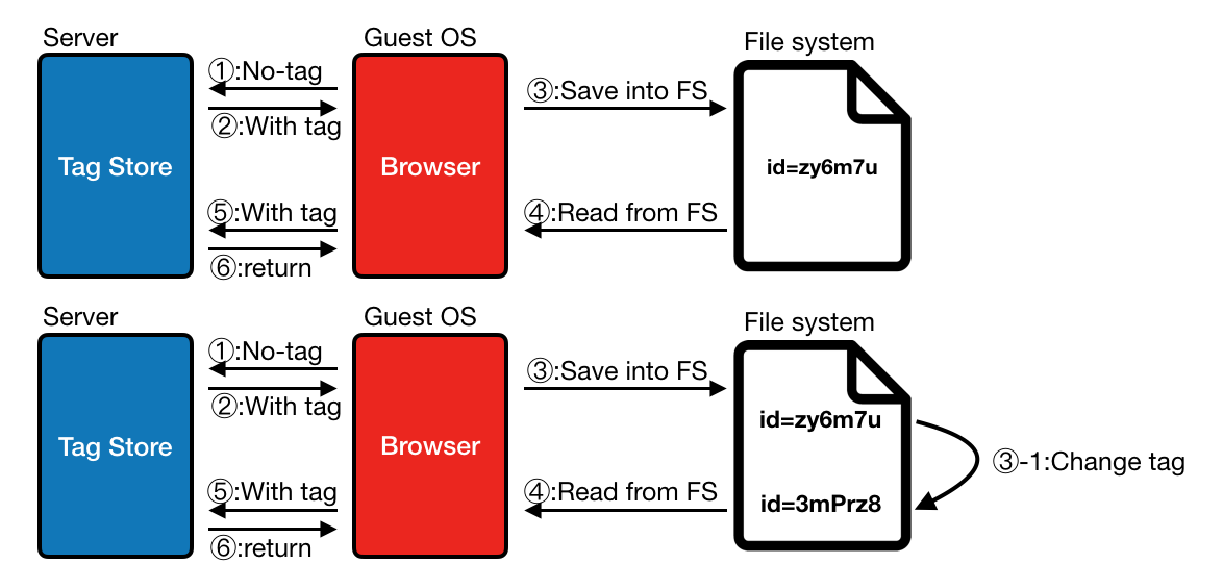
\includegraphics[width=8cm]{img/tag.eps}
\caption{ユーザトラッキングとタグプロテクション。上のイメージはブラウザが一回目と二回目の訪問する時に一部の個人識別子の移動ディレクション。一回目はタグないからサーバが生成して、サーバのストレージとクライアント同時に保存する。下のイメージは個人識別子を保護する時に、一回目と二回目の訪問する間で個人識別子をなんかの手段で直す。}
\label{figure:tag}
\end{center}
\end{figure}


\section{差分内容の保護と隔離}
\label{cha:protect}
トラッキングに使われる嫌疑があったタグを二回目サーバを訪問する時に、サーバが正しい認識できないような形に変える必要がある。図\ref{figure:tag}のように、一回目の通信で生成した新しいタグをそして、タグの隔離効果をテストするため、修正前の元のタグはホストに保存しなければならない。ファイルとネットワーク通信の差分の対応は違う。

\subsection{ファイルの差分の対応}
ファイルの差分内容は全部diffコマンドで見つかったから、出力ファイルは解析し、オリジナルファイルのふさわしい部分を処理する必要がある。ファイルの形によって処理手段は違うから、次のように扱う。

\begin{description}
\item{・テキストファイル: }
テキストファイルの対応は、まずdiffの出力ラインから差分タグを検出、差分タグを双子の環境の各ホスト環境のストレージに保存する。それからファイル名でゲストOSのファイルシステムに対応したファイルをawkで差分タグを直す。直したタグは直した前のタグと同じように保存する。タグの変更は、乱数を生成、元のタグと同じ形式に変わって、コンテナFSに書き込む。よく使われたタグの形式はBase64、Hash(MD5,SHA256)、UUIDなどの形式がある。それらのタグをふさわしいランダムジェナレータで取って代わり、タグの保護ができる。
\item{・データベース: }
テキストファイルと同じように差分タグを検出、保存する。タグの直すはawkではなく、データベースの管理ツールを利用して簡単で直せる。関係型データベースはSQLのupdateを利用し、No-SQLは直接にKey-Valueを直す。
\item{・バイナリファイル: }
バイナリファイルの差分は直接的にdiffコマンドを使うのができないから、バイナリファイル中のテキストの部分を引き出して差分を取る。
\end{description}
\subsection{ネットワーク通信の差分の対応}
ネットワークの通信の差分タグは通信中にMITM-Proxyによるファイルシステムに保存する。保存の形は節\label{sec:net}のようにテキストファイルに保存して、diffコマンドで差分を取る。取り除いた差分タグはファイルの差分内容と同じようにホストのストレージに保存する。








 
 
\begin{table*}[ht]
\caption{差分がないファイルと差分があるファイルの数}
\centering
\begin{tabular}{|p{2cm}|l|p{1.9cm}|p{1.9cm}|l|p{1.9cm}|p{1.9cm}|}
\hline
&\multicolumn{3}{|c|}{\footnotesize{Firefox}}&\multicolumn{3}{c|}{\footnotesize{Google Chrome}}\\
\hline
&\multirow{2}{1.5cm}{\footnotesize{個人情報がない}} &
\multicolumn{2}{c|}{\footnotesize{差分がある}} &\multirow{2}{1.5cm}{\footnotesize{個人情報がない}}&
\multicolumn{2}{c|}{\footnotesize{差分がある}} \\
\cline{3-4}\cline{6-7}
  & & \footnotesize{不明なバイナリ} & \footnotesize{テキストと扱えるバイナリ(行数)}& &\footnotesize{不明なバイナリ} & \footnotesize{テキストと扱えるバイナリ(行数)} \\
\hline
\footnotesize{更新されたファイル}&\multicolumn{1}{r|}{\footnotesize{52}}&\multicolumn{1}{r|}{\footnotesize{0}}&\multicolumn{1}{r|}{\footnotesize{7(28)}}  & \multicolumn{1}{r|}{\footnotesize{98}} & \multicolumn{1}{r|}{\footnotesize{5}} & \multicolumn{1}{r|}{\footnotesize{47(114)}} \\
\hline
\footnotesize{乱数生成器の置き換え}&\multicolumn{1}{r|}{\footnotesize{55}}&\multicolumn{1}{r|}{\footnotesize{0}}&\multicolumn{1}{r|}{\footnotesize{4(10)} }& \multicolumn{1}{r|}{\footnotesize{128} }& \multicolumn{1}{r|}{\footnotesize{5} }& \multicolumn{1}{r|}{\footnotesize{17(46)}} \\
\hline
\footnotesize{ローカルタイムスタンプの固定}&\multicolumn{1}{r|}{\footnotesize{55}}&\multicolumn{1}{r|}{\footnotesize{0}}&\multicolumn{1}{r|}{\footnotesize{4(8)} }&  \multicolumn{1}{r|}{\footnotesize{128} }& \multicolumn{1}{r|}{\footnotesize{5} }&\multicolumn{1}{r|}{\footnotesize{17(41) }}\\
\hline
\footnotesize{前処理後}&\multicolumn{1}{r|}{\footnotesize{55}}&\multicolumn{1}{r|}{\footnotesize{0}}&\multicolumn{1}{r|}{\footnotesize{4(8)}} &\multicolumn{1}{r|}{ \footnotesize{136} }& \multicolumn{1}{r|}{\footnotesize{5} }&\multicolumn{1}{r|}{\footnotesize{9(15)}}\\
\hline
\end{tabular}
\label{fig:result}
\end{table*}

\begin{table*}[ht]



\caption{ファイルの差分の例}
\centering

\begin{tabular}{ |l|p{6cm}|p{6cm}| }

 \hline
 \footnotesize{ファイル名} &\footnotesize{コンテナ1} &\footnotesize{コンテナ2}\\
 \hline
 \footnotesize{cookies.sqlite} & \footnotesize{value = 132=S1fjWe4xjUJJowuImYQyi...} & \footnotesize{value = 132=ablTT1GOqBlYlBX-MQ...}\\
\hline
 \footnotesize{places.sqlite} & \footnotesize{guid = xhIxtPu6zAJ7} & \footnotesize{guid = IlfETnEs0Dr4}\\
\hline
 \footnotesize{sessionstore.js} & \footnotesize{"docshellUUID": "\{4c4508da-9468-430b-8eac- 0484dcc43e5d\}"} & \footnotesize{"docshellUUID": "\{bfcff6ba-42c2-4731-a65c- ae1ba7b1cc0e\}"}\\
 \hline
\footnotesize{prefs.js} & \footnotesize{user\_pref("browser.slowStartup.averageTime", 14971)} & \footnotesize{user\_pref("browser.slowStartup.averageTime", 18103)}\\
\hline
\end{tabular}
\label{fig:data}
\end{table*}

\begin{table*}[ht]
\caption{ネットワーク通信の差分の例}
\centering

\begin{tabular}{ |p{3.5cm}|p{5cm}|p{5cm}| }

 \hline
 \footnotesize{URL} &\footnotesize{コンテナ1} &\footnotesize{コンテナ2}\\
 \hline
 \footnotesize{www.google.com} & \footnotesize{Cookie:1P\_JAR=2017-12-12-04,NID=119=BGA6eL4YT9Q...} & \footnotesize{Cookie:1P\_JAR=2017-12-12-04,NID=rzmrga\_L3s...}\\
\hline
 \footnotesize{www.google.com/gen\_204} & \footnotesize{ei:pdcsW5TSLIb28AXosLGYBA} & \footnotesize{ei:pdcsW-vCDMfS8QWq-I34Bg}\\
\hline
 \footnotesize{ssl.gstatic.com/gb/ima ges/i1\_1967ca6a.png} & \footnotesize{age:253629} & \footnotesize{age:253628}\\
 \hline

\end{tabular}
\label{fig:data}
\end{table*}








\section{実験}
\subsection{双子のブラウザが生成したファイルの差分}
\label{sec:file}

本研究室ではFirefoxとGoogle Chromeで双子のブラウザを実装している。今回、ユーザトラッキングを行っている代表的なWebサイトとしてGoogleを選択しhttp://www.google.com/を訪問する実験を行った。これは、ログインを必要としない簡単なサイトである。

\subsubsection{Firefox}
まずFirefoxブラウザを双子のブラウザとして双子の環境で実行した。コンテナの全てのファイルの変化をリストアップしたところ、全部で59個のファイルが作成された。その中に29個が~/.cacheにある一時的なファイルのためファイル名によるフィルタにより自動的に除外された。残る30個のファイルに対して前処理を行って、テキスト化しdiffコマンドで差分を取った結果は全部28行であった。\ref{cha:file}章で述べた方法に従ってテキスト化した差分を削減した結果、最終的に差分は8行だった。識別できないバイナリファイルはなかった。

表\ref{fig:data}に、発見した差分の一部を示す。cookies.sqliteには、HTTP Cookiesが保存されていることがわかる。places.sqliteは、訪問履歴を保持するファイルである。その中に、アクセスしたURLが保存されている。このように、URLの中に、ユーザトラッキングに利用可能なタグが埋め込まれていることがわかる。

この実験の結果、提案手法により、ファイルを特定し、使用者の識別子を検出することができ、ユーザトラッキングに使われる個人識別情報が含まれることが確認された。

\subsubsection{Chrome}

2番目の実験はGoogle Chromeで行った。結果を表\ref{fig:result}に表す。差分があるファイルはFirefoxより多い。識別できないバイナリファイルが5個残された。

\label{sec:one}
\subsection{ネットワーク通信内容の差分}
ブラウザが行うネットワーク通信の内容の差分を調査した。訪問したサイトは、\ref{sec:file}節と同じである。

全部の通信の数は21個あり、テキスト形式のファイル以外にpngが6個、icoが1個あった。20個のメッセージの内容に差分があり、1番目の通信だけは差分がなかった。ネットワーク通信の差分はタイムスタンプと重複を除き全部で22行あった。応答メッセージの内容に差分があるファイルが2個あった。それらのURLはwww.google.comとwww.google.com/gen\_204であった。また、URLが違う通信の数は3個あった。

メッセージの内容にはcookiesが現れている。これは、cookies.sqlite(表\ref{fig:data})にも含まれている。



\subsection{プライバシ保護の評価}

上記の実験で検出した個人情報データは、\ref{cha:protect}節で紹介した方法でタグの引き換え、及び削除でプライバシを保護したい。保護する結果の評価は前と同じように双子の環境で動き、図\ref{figure:secres}のように、双子のブラウザで訪問を二回行って、保護する結果は成功かどうかでテストする。もし二回目のQueryの結果に一回目のQuery内容が含まれば、タグの保護がうまう行かなっかたと表す。

\subsubsection{コンテナオペレーション}


\begin{figure}[ht]
\begin{center}
\includegraphics[width=8cm]{img/secres.eps}
\caption{個人識別子を保護する結果の評価。一回目の訪問する時に、ブラウザがキーワード「A」を入力し、サーバに送信する結果は、すべてA関連のデータである。二回目の訪問にはキーワード「B」を入力が、もし結果には"A"の結果が出れば個人識別子はよく保護していないとわかる}
\label{figure:secres}
\end{center}
\end{figure}


\section{関連研究}
Qubes-OS\cite{qubes}は高いセキュリティを実現するためのOSである。 Qubes-OSは仮想計算機モニタ(Xen)を用いて、アプリケーションを隔離された仮想実行環境で実行する。Qubes-OSには、複数の仮想実行環境のファイルを比較する機能はない。

Blink-Docker\cite{blink}はコンテナ中でブラウザを実行することで、Canvas Fingerprintを利用したユーザトラッキングからユーザを保護する。Canvas Fingerprint はハードウェアや OS のわずかな違いによってクライアントを特定する手法である。Blink-Dockerはコンテナ技術を利用し、毎回 Fingerprint を変えることができる。本研究では、通信内容を検査し、そのようなユーザトラッキングを検出したいと考えている。



\section{まとめ}
本研究では人間の双子の研究に参考した双子の環境を提案した。本研究ではDockerコンテナを利用し、軽量で類似の仮想環境を作り、ファイルと通信内容に含まれる個人情報を検出する。

本研究室で開発された双子のブラウザを双子の環境で実行し、それらが生成するファイルの差分を調査するツールを実装した。また、Man-In-The-Middle Proxyを用いて、通信内容を比較するツールを実装した。実装した双子のブラウザを利用し、個人情報と個人識別子である可能性が高いユニークなタグがいくつ検出した。そして、個人識別子を変更の方で保護する。

%%%%%%%%%%%%%%%%%%%%%%%
%% ここまで本文
%%%%%%%%%%%%%%%%%%%%%%%


%%FIXME
%%bibファイルを指定する
\begin{thebibliography}{1}

\bibitem{qubes}
 {\small Qubes OS - A reasonably secure operating system: https://www.qubes-os.org/, accessed: 2017-11-22.}
\bibitem{blink}
 P Laperdrix, W Rudametkin, B Baudry: "Blink: A moving-target approach to fingerprint diversification" 37th IEEE Symposium on Security and Privacy, Poster Session, [Online]
http://www.ieee-security.org/TC/SP2016/poster-abstracts/59-poster\_abstract.pdf,  (2016).
\bibitem{dynamic}
Javier Verd, Juan Jos Costa, Alex Pajuelo: "Dynamic Web worker pool management for highly parallel javascript web applications" Concurrency and Computation: Practice and Experience, 28(13):35253539, September 2015.
\bibitem{comsys}
張 世申,新城 靖,三村 賢次郎: "個人情報を含むファイルと通信を検出ための双子の環境の提案",情報処理学会第29回コンピュータシステムシンポジウム ポスターセッション, 2ページ(2017).
\bibitem{web}
三村 賢次郎,新城 靖,張 世申: "Webサービスごとに隔離されたブラウジング環境の提案", 同上.
\end{thebibliography}

\end{document}
